%
%
% UCSD Doctoral Dissertation Template
% -----------------------------------
% http://ucsd-thesis.googlecode.com
%
%
% ----------------------------------------------------------------------
% WARNING: 
%
%   This template has not endorced by OGS or any other official entity.
%   The official formatting guide can be obtained from OGS.
%   It can be found on the web here:
%   http://ogs.ucsd.edu/AcademicAffairs/Documents/Dissertations_Theses_Formatting_Manual.pdf
%
%   No guaranty is made that this LaTeX class conforms to the official UCSD guidelines.
%   Make sure that you check the final document against the Formatting Manual.
%  
%   That being said, this class has been routinely used for successful 
%   publication of doctoral theses.  
%
%   The ucsd.cls class files are only valid for doctoral dissertations.
%
%
% ----------------------------------------------------------------------
% GETTING STARTED:
%
%   Lots of information can be found on the project wiki:
%   http://code.google.com/p/ucsd-thesis/wiki/GettingStarted
%
%
%   To make a pdf from this template use the command:
%     pdflatex template
%
%
%   To get started please read the comments in this template file 
%   and make changes as appropriate.
%
%   If you successfully submit a thesis with this package please let us
%   know.
%
%
% ----------------------------------------------------------------------
% KNOWN ISSUES:
%
%   Currently only the 12pt size conforms to the UCSD requirements.
%   The 10pt and 11pt options make the footnote fonts too small.
%
%
% ----------------------------------------------------------------------
% HELP/CONTACT:
%
%   If you need help try the ucsd-thesis google group:
%   http://groups.google.com/group/ucsd-thesis
%
%
% ----------------------------------------------------------------------
% BUGS:
%
%   Please report all bugs at:
%   http://code.google.com/p/ucsd-thesis/issues/list
%
%
% ----------------------------------------------------------------------
% More control of the formatting of your thesis can be achieved through
% modifications of the included LaTeX class files:
%
%   * ucsd.cls    -- Class file
%   * uct10.clo   -- Configuration files for font sizes 10pt, 11pt, 12pt
%     uct11.clo                            
%     uct12.clo
%
% ----------------------------------------------------------------------



% Setup the documentclass 
% default options: 12pt, oneside, final
%
% fonts: 10pt, 11pt, 12pt -- are valid for UCSD dissertations.
% sides: oneside, twoside -- note that two-sided theses are not accepted 
%                            by OGS.
% mode: draft, final      -- draft mode switches to single spacing, 
%                            removes hyperlinks, and places a black box
%                            at every overfull hbox (check these before
%                            submission).
% chapterheads            -- Include this if you want your chapters to read:
%                              Chapter 1
%                              Title of Chapter
%
%                            instead of
%                              1 Title of Chapter
\documentclass[12pt,chapterheads]{ucsd}



% Include all packages you need here.  
% Some standard options are suggested below.
%
% See the project wiki for information on how to use 
% these packages. Other useful packages are also listed there.
%
%   http://code.google.com/p/ucsd-thesis/wiki/GettingStarted



%% AMS PACKAGES - Chances are you will want some or all 
%    of these if writing a dissertation that includes equations.
%  \usepackage{amsmath, amscd, amssymb, amsthm}

%% GRAPHICX - This is the standard package for 
%    including graphics for latex/pdflatex.
\usepackage{scrextend}
\usepackage{pslatex}
\usepackage{graphicx}

%% CAPTION
% This overrides some of the ugliness in ucsd.cls and
% allows the text to be double-spaced while letting figures,
% tables, and footnotes to be single-spaced--all OGS requirements.
% NOTE: Must appear after graphics and ams math
\makeatletter
\gdef\@ptsize{2}% 12pt documents
\let\@currsize\normalsize
\makeatother
\usepackage{setspace}
\doublespace
\usepackage[font=small, width=0.9\textwidth]{caption}

%% SUBFIG - Use this to place multiple images in a
%    single figure.  Subfig will handle placement and
%    proper captioning (e.g. Figure 1.2(a))
% \usepackage{subfig}

%% TIMES FONT - replacements for Computer Modern
%%   This package will replace the default font with a
%%   Times-Roman font with math support.
% \usepackage[T1]{fontenc}
% \usepackage{mathptmx}

%% INDEX
%   Uncomment the following two lines to create an index: 
% \usepackage{makeidx}
% \makeindex
%   You will need to uncomment the \printindex line near the
%   bibliography to display the index.  Use the command
% \index{keyword} 
%   within the text to create an entry in the index for keyword.
%   To compile a LaTeX document with an index the 'makeindex'
%   command will need to be run.  See the wiki for more details.

%% HYPERLINKS
%   To create a PDF with hyperlinks, you need to include the hyperref package.
%   THIS HAS TO BE THE LAST PACKAGE INCLUDED!
%   Note that the options plainpages=false and pdfpagelabels exist
%   to fix indexing associated with having both (ii) and (2) as pages.
%   Also, all links must be black according to OGS.
%   See: http://www.tex.ac.uk/cgi-bin/texfaq2html?label=hyperdupdest
%   Note: This may not work correctly with all DVI viewers (i.e. Yap breaks).
%   NOTE: hyperref will NOT work in draft mode, as noted above.
% \usepackage[colorlinks=true, pdfstartview=FitV, 
%             linkcolor=black, citecolor=black, 
%             urlcolor=black, plainpages=false,
%             pdfpagelabels]{hyperref}
% \hypersetup{ pdfauthor = {Your Name Here}, 
%              pdftitle = {The Title of The Dissertation}, 
%              pdfkeywords = {Keywords for Searching}, 
%              pdfcreator = {pdfLaTeX with hyperref package}, 
%              pdfproducer = {pdfLaTeX} }
% \urlstyle{same}
% \usepackage{bookmark}


%% CITATIONS
% Sets citation format
% and fixes up citations madness
\usepackage{microtype}  % avoids citations that hang into the margin


%% FOOTNOTE-MAGIC
% Enables footnotes in tables, re-referencing the same footnote multiple times.
\usepackage{footnote}
\makesavenoteenv{tabular}
\makesavenoteenv{table}


%% TABLE FORMATTING MADNESS
% Enable all sorts of fun table tricks
\usepackage{rotating}  % Enables the sideways environment (NCPW)
\usepackage{array}  % Enables "m" tabular environment http://ctan.org/pkg/array
\usepackage{booktabs}  % Enables \toprule  http://ctan.org/pkg/array


%% INCLUDING PDFS
% Arguments:
% - draft -- use a black box for rendering speed
\usepackage{pdfpages}
% Options for \includepdf and \includepdfmerge:
% pages={1-2,3,4} or pages=- for all
% frame -- outline with a black box
% noautoscale -- don't resize pages, allowing for use with the graphicsx \scale command
% Global options:
\includepdfset{pages={-},noautoscale,fitpaper=false,pagecommand=\thispagestyle{plain},frame}

\begin{document}

%% FRONT MATTER
%
%  All of the front matter.
%  This includes the title, degree, dedication, vita, abstract, etc..
%  Modify the file template_frontmatter.tex to change these pages.
%
%
% UCSD Doctoral Dissertation Template
% -----------------------------------
% http://ucsd-thesis.googlecode.com
%
%


%% REQUIRED FIELDS -- Replace with the values appropriate to you

% No symbols, formulas, superscripts, or Greek letters are allowed
% in your title.
\title{The Title Of The Dissertation}

\author{Your Name Here}
\degreeyear{\the\year}

% Master's Degree theses will NOT be formatted properly with this file.
\degreetitle{Doctor of Philosophy}

\field{Mathematics}
\specialization{Anthropogeny}  % If you have a specialization, add it here

\chair{Professor Chair Master}
% Uncomment the next line iff you have a Co-Chair
% \cochair{Professor Cochair Semimaster}
%
% Or, uncomment the next line iff you have two equal Co-Chairs.
%\cochairs{Professor Chair Masterish}{Professor Chair Masterish}

%  The rest of the committee members  must be alphabetized by last name.
\othermembers{
Professor Humor Less\\
Professor Ironic Name\\
Professor Cirius Thinker\\
}
\numberofmembers{4} % |chair| + |cochair| + |othermembers|


%% START THE FRONTMATTER
%
\begin{frontmatter}

%% TITLE PAGES
%
%  This command generates the title, copyright, and signature pages.
%
\makefrontmatter

%% DEDICATION
%
%  You have three choices here:
%    1. Use the ``dedication'' environment.
%       Put in the text you want, and everything will be formated for
%       you. You'll get a perfectly respectable dedication page.
%
%
%    2. Use the ``mydedication'' environment.  If you don't like the
%       formatting of option 1, use this environment and format things
%       however you wish.
%
%    3. If you don't want a dedication, it's not required.
%
%
\begin{dedication}
  To two, the loneliest number since the number one.
\end{dedication}


% \begin{mydedication} % You are responsible for formatting here.
%   \vspace{1in}
%   \begin{flushleft}
% 	To me.
%   \end{flushleft}
%
%   \vspace{2in}
%   \begin{center}
% 	And you.
%   \end{center}
%
%   \vspace{2in}
%   \begin{flushright}
% 	Which equals us.
%   \end{flushright}
% \end{mydedication}



%% EPIGRAPH
%
%  The same choices that applied to the dedication apply here.
%
\begin{epigraph} % The style file will position the text for you.
  \emph{A careful quotation\\
  conveys brilliance.}\\
  ---Smarty Pants
\end{epigraph}

% \begin{myepigraph} % You position the text yourself.
%   \vfil
%   \begin{center}
%     {\bf Think! It ain't illegal yet.}
%
% 	\emph{---George Clinton}
%   \end{center}
% \end{myepigraph}


%% SETUP THE TABLE OF CONTENTS
%
\tableofcontents
\listoffigures  % Comment if you don't have any figures
\listoftables   % Comment if you don't have any tables



%% ACKNOWLEDGEMENTS
%
%  While technically optional, you probably have someone to thank.
%  Also, a paragraph acknowledging all coauthors and publishers (if
%  you have any) is required in the acknowledgements page and as the
%  last paragraph of text at the end of each respective chapter. See
%  the OGS Formatting Manual for more information.
%
\begin{acknowledgements}
 Thanks to whoever deserves credit for Blacks Beach, Porters Pub, and
 every coffee shop in San Diego.

 Thanks also to hottubs.
\end{acknowledgements}


%% VITA
%
%  A brief vita is required in a doctoral thesis. See the OGS
%  Formatting Manual for more information.
%
\begin{vitapage}
\begin{vita}
  \item[2002] B.~S. in Mathematics \emph{cum laude}, University of Southern North Dakota, Hoople
  \item[2002-2007] Graduate Teaching Assistant, University of California, San Diego
  \item[2007] Ph.~D. in Mathematics, University of California, San Diego
\end{vita}
\begin{publications}
  \item Your Name, ``A Simple Proof Of The Riemann Hypothesis'', \emph{Annals of Math}, 314, 2007.
  \item Your Name, Euclid, ``There Are Lots Of Prime Numbers'', \emph{Journal of Primes}, 1, 300 B.C.
\end{publications}
\end{vitapage}


%% ABSTRACT
%
%  Doctoral dissertation abstracts should not exceed 350 words.
%   The abstract may continue to a second page if necessary.
%
\begin{abstract}
  This dissertation will be abstract.
\end{abstract}


\end{frontmatter}






%% DISSERTATION

% A common strategy here is to include files for each of the chapters. I.e.,
% Place the chapters is separate files: 
%   chapter1.tex, chapter2.tex
% Then use the commands:
%   \include{chapter1}
%   \include{chapter2}
%
% Of course, if you prefer, you can just start with
%   \chapter{My First Chapter Name}
% and start typing away.  
\chapter{Just a Test}
This is only a test.
\section{A section}
Lorem ipsum dolor sit amet, consectetuer adipiscing elit. Nulla odio
sem, bibendum ut, aliquam ac, facilisis id, tellus. Nam posuere pede
sit amet ipsum. Etiam dolor. In sodales eros quis pede.  Quisque sed
nulla et ligula vulputate lacinia. In venenatis, ligula id semper
feugiat, ligula odio adipiscing libero, eget mollis nunc erat id orci.
Nullam ante dolor, rutrum eget, vestibulum euismod, pulvinar at, nibh.
In sapien. Quisque ut arcu. Suspendisse potenti. Cras consequat cursus
nulla.

\subsection{A Figure Example}
\label{ssec:figure_example}

This subsection shows a sample figure.

\begin{figure}[h] 
  \centering
  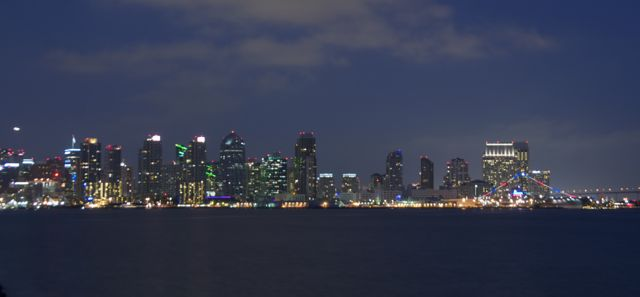
\includegraphics[width=0.5\textwidth]{sandiego}
  \caption[Short figure caption (must be \protect{$< 4$} lines in the list of figures)]{A picture of San Diego.  Note that figures must be on their own line (no neighboring text) and captions must be single-spaced and appear \protect\textit{below} the figure.  Captions can be as long as you want, but if they are longer than 4 lines in the list of figures, you must provide a short figure caption.\index{SanDiego}} 
  \label{fig:sandiego}
\end{figure}

\subsection{A Table Example}

While in Section \ref{ssec:figure_example} Figure \ref{fig:sandiego} we had a majestic figure, here we provide a crazy table example.


%%%% TABLE 1 %%%%
\vspace{0.25in}
\begin{table}[!ht]
\caption[Short figure caption (must be \protect{$< 4$} lines in the list of tables)]{A table of when I get hungry.  Note that tables must be on their own line (no neighboring text) and captions must be single-spaced and appear \protect\textit{above} the table.  Captions can be as long as you want, but if they are longer than 4 lines in the list of figures, you must provide a short figure caption.}

\vspace{-0.25in}
\begin{center}
\begin{tabular}{|p{1in}|p{2in}|p{3in}|}

\hline
Time of day & Hunger Level & Preferred Food \\

\hline
8am & high & IHOP (French Toast) \\

\hline
noon & medium & Croutons (Tomato Basil Soup \& Granny Smith Chicken Salad) \\

\hline
5pm & high & Bombay Coast (Saag Paneer) or Hi Thai (Pad See Ew) \\

\hline
8pm & medium & Yogurt World (froyo!) \\

\hline
\end{tabular}
\end{center}
\label{tab:analysis3}
\end{table}

\chapter{Structure Comparison}

\includepdf{Bioinformatics_2010_Prlic_.pdf}

%% APPENDIX
\appendix
\chapter{Final notes}
What to do about things \cite{Martin_1983}.  What did he say \cite{Rilling_Insel_1999}.
  Remove me in case of abdominal pain.



%% END MATTER
% \printindex %% Uncomment to display the index
% \nocite{}  %% Put any references that you want to include in the bib 
%               but haven't cited in the braces.
\bibliographystyle{alpha}  %% This is just my personal favorite style. 
%                              There are many others.
%\setlength{\bibleftmargin}{0.25in}  % indent each item
%\setlength{\bibindent}{-\bibleftmargin}  % unindent the first line
%\def\baselinestretch{1.0}  % force single spacing
%\setlength{\bibitemsep}{0.16in}  % add extra space between items
\bibliography{template}  %% This looks for the bibliography in template.bib 
%                          which should be formatted as a bibtex file.
%                          and needs to be separately compiled into a bbl file.
\end{document}